\chapter{MANO Scalability}
\label{ch:Scalability}

In this chapter we discuss the two directions we explored to investigate MANO orchestrator scalability. First, we discuss the scalability plugin that was added to pishahang. The scalability plugin adds 3 main functionalities to pishahang, 1) spawn new child instances of pishahang by allocating new physical resources, 2) Redirecting requests from parent MANO to the child instances and 3) managing the state of child instances. Second, we discuss the experiments conducted on OSM and Pishahang to understand the resource utilization. We also propose a more generic framework to characterize and analyze MANO under load.

\section{Introduction}

\todo[inline]{Add content}

\subsection{Definition of scaling}
`Scalability' is defined in different ways in various academic work. Some of the definitions are listed below.
\begin{itemize}	 
	
	\item "The ability of a particular system to fit a problem as the scope of that problem increases (number of elements or objects, growing volumes of work and/or being susceptible to enlargement)." \cite{furht_handbook_2010}
	
	\item "Scalability of service is a desirable property of a service which provides an ability to handle growing amounts of service loads without suffering significant degradation in relevant quality attributes. The scalability enhanced by scalability assuring schemes such as adding various resources should be proportional to the cost to apply the schemes." \cite{lee_software_2010}
	
	\item "Scalability is the ability of an application to be scaled up to meet demand through replication and distribution of requests across a pool or farm of servers." \cite{chieu_scalability_2011}
	
	\item "A system is said to be scalable if it can handle the addition of users and resources without suffering a noticeable loss of performance or increase in administrative complexity" \cite{noauthor_scale_nodate}
	
\end{itemize}

\subsection{Why does a MANO need scaling?}
\paragraph{}
In recent years, distributed systems have gained an increase in the number of users and resources. Scaling such a system is an important aspect when large user requests have to be served without compromising system performance or increase in administrative complexity. In terms of MANO, when there are a large number Network Service(NS) instantiation of various network functions, they need to be instantiated considering all the relevant metrics of the system.

\paragraph{System load:}
In a distributed system, the system load is the large amount of data that is to be managed by network services increasing the total number of requests for service.
The load on a MANO can be defined in terms of it's load on NFV Orchestrator (NFVO) to process large number of tasks like on-boarding, instantiation and monitoring of VNFs. The NFVO of a MANO receives monitoring information which also increases the load on NFVO triggering it to scale the network service across multiple MANOs in a distributed system \cite{soenen2017optimising}.


\paragraph{Lifecycle Management \& service provisioning:} To provision a network service, the NFVO of a MANO's functionality include instantiation, global resource management scaling in/out , event correlation and termination of services. These functionalities form the lifecycle of NS. With the increase in instantiation of NS over a distributed network, the lifecycle management of each service is a overhead, hence increasing the provision time. This can be better handled when the MANO can be scaled out. To manage services with a closer proximity of geographical region, MANOs could be scaled in.


\section{Scalability Plugin}

MANO framework faces scalability challenges in large-scale deployments. The amount of infrastructure a single instance of MANO framework can manage is limited. The scaling of MANO should be addressed to avoid it from being the bottleneck in the NFV paradigm. \\

We propose a hierarchical scaling mechanism for MANO by implementing and evaluating a scalability plugin (SPL) in pishahang. SPL adds the following features to pishahang 1) Spawn/Terminate child MANO instances, 2) State management between instances, 3) Redirection of requests from parent instance to child instances and 4) Monitoring of system load on all instances

\subsection{Architecture}

SPL is built based on the "base plugin framework" of SONATA. The figure \ref{fig:pmdesign} from SONATA documentation shows the high-level architecture of the SONATA MANO framework. The plugins communicate over the message broker using AMQP with other plugins and together facilitate the functions of MANO.

\begin{figure}[h]
	\centering
	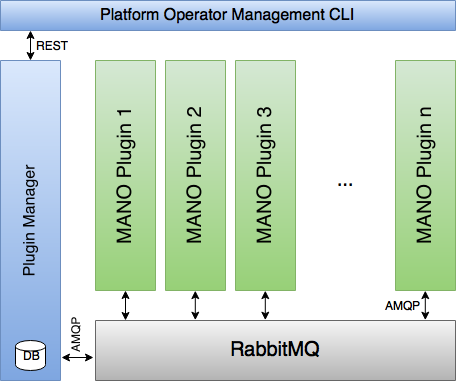
\includegraphics[width=0.7\linewidth]{figures/pm_design}
	\caption{SONATA MANO plugin architecture}
	\label{fig:pmdesign}
\end{figure}

The architecture of the scalability plugin is shown in the figure \ref{fig:scalingarch}. SPL mainly consists of 1) \textbf{Scaling Manager:} is responsible for the overall workflow of the SPL, which includes monitoring, spawning, termination and state management of MANO instances. 2) \textbf{MANO Manager:} is responsible for sending the on-boarding and instantiation requests to the parent MANO using python-mano-wrappers. SPL co-ordinates with the service lifecycle management plugin in pishahang to provide the features discussed above. The workflow of this is discussed in the further sections. 

\subsubsection{Scaling Manager}

Features of the scaling manager are discussed briefly in this section. 

\subsubsection*{Monitoring}

SPL needs to continuously monitor the system resource utilization and take scaling decisions based on that. We are using the \textit{average system load} values given by the linux kernel for taking the scaling decisions. System load is the number of processes which are being executed by the CPU or in waiting state. The linux kernel provides 3 average values of system load calculated over a period of 1, 5 and 15 minutes. \\

As a proof of concept, SPL uses \textit{5m} and \textit{15m} moving averages as a heuristic for scaling decisions. \textit{1m} average is not considered to avoid taking decisions on a short lived spike in system load. SPL has the following simple rule set listed below, note that the configurable threshold value is used to take relevant actions. For simplicity, we consider "0.7" as the threshold value as it is generally used in the wild by system administrators. 

\begin{enumeratelist}

\begin{itemize}
	\item{\textbf{Rule 1}\\} If \textit{5m} load average is more than the \textit{threshold} value, then, SPL will consider this as a warning sign and start preparing a child MANO instance.
	\item{\textbf{Rule 2}\\} If \textit{15m} load average is more than the \textit{threshold} value, then, SPL will consider this as a critical sign and start redirecting service requests on the parent mano to the child MANO instance.
	\item{\textbf{Rule 3}\\} If \textit{15m} load average of both the parent and child instances are less than the \textit{threshold} value, then, SPL will consider this as decreasing load and terminate the child MANO instance.

\end{itemize}
\caption{Scaling Plugin Rules}
\label{list:splrules}
\end{enumeratelist}


\subsubsection*{SLM Communication}

The monitoring of the load information happens in the SPL, however, the service requests are handled by the SLM plugin. SLP communicates information about the current load of the instances to the SLM and based on this response, SLM decides whether to continue serving the request or to forward it to one of the child MANOs.

The forwarding logic is implemented on the SLM plugin of pishahang. The forwarding logic includes on-boarding the VNFD/NSD and instantiating it.

\subsubsection*{Spawning}

Spawning refers to the action of instantiating a child instance of pishahang by allocating new physical resources on existing infrastructure. According to Rule 1 from \ref{list:splrules}, when the threshold is reached, a request to instantiate a new instance is sent to the Mano Manager. Mano Manager will instantiate a new instance of pishahang and returns the IP address of the newly deployed instance. This new instance is now added to the list of child MANO instances and continuously monitored.
 

\subsubsection*{Termination}

Once the load on the parent MANO and child MANO instances are reducing, it becomes unnecessary and expensive to use the allocated physical resources of the child MANO. According to Rule 3 from \ref{list:splrules}, the termination request of the child MANO is sent to the MANO Manager and the metadata generated by the child instances are saved on the parent instance. Metadata that is saved includes the VNF records and network service records.


\subsubsection{MANO Manager}
MANO Manager is responsible for the end communication with the parent MANO. MANO Manager receives an instantiation request from the Scaling Manager and uses python-mano-wrappers to make an instantiation request to the parent MANO to instantiate a child MANO instance. 

MANO Manager will wait for successful instantiation of the instance and return the IP address of the instance to the Scaling Manager.

\subsubsection*{Service Descriptors}

We designed a basic function descriptor and service descriptor in the schema supported by the pishahang MANO framework. The descriptors are stored as part of the scaling plugin and used by the MANO Manager to on-board and instantiate upon request. We have created the descriptors for both OSM and Pishahang.

\subsubsection*{MANO Image}

A Virtual Machine (VM) image with MANO pre-installed is used along with the service descriptors to spawn new instances of MANO. As a proof of concept, we have created images with OSM and pishahang. However, the pishahang image that was created was unstable and has unexpected behavior. These images are first created locally and later uploaded to the VIM where the instances will be created. In our tests we used OpenStack as the VIM.

\begin{figure}[h]
	\centering
	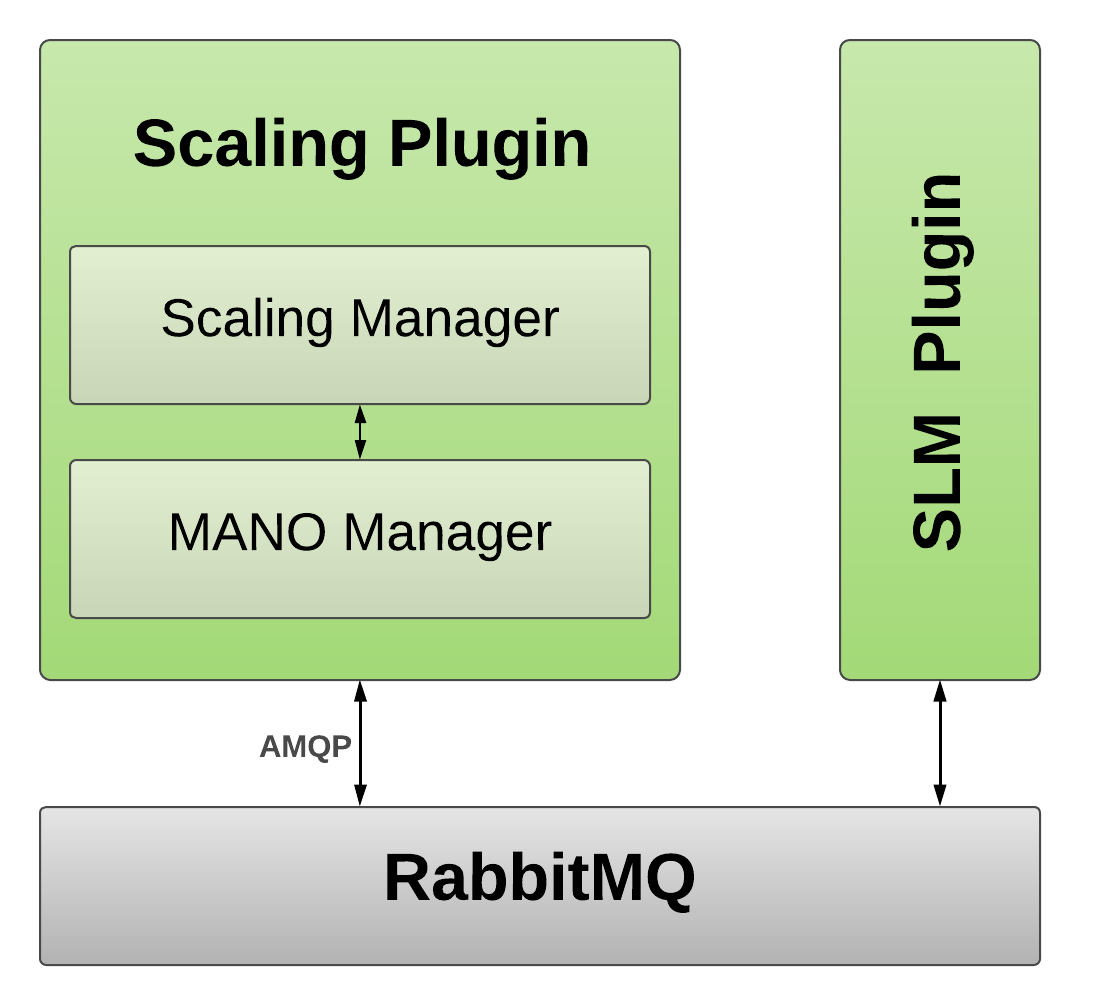
\includegraphics[width=0.7\linewidth]{figures/scalingarch}
	\caption{Scaling plugin architecture}
	\label{fig:scalingarch}
\end{figure}


\subsection{Workflow}

\subsubsection{SLM with SLP}

The workflow of how the SLM and SLP interacts is shown in the figure \ref{fig:slpslmworkflow}. At first, an instantiation request comes into the parent mano instance and this is first seen at SLM. SLM will then request SLP for the current system load status. If the parent MANO is loaded, SLP will reply with the details of the child MANO instance, which will then be used by SLM to redirect the incoming request by on-boarding and instantiating the network service on the child instance. If the parent MANO is not loaded, then, SLM will continue its normal flow to deploy the network service

\begin{figure}[h]
	\centering
	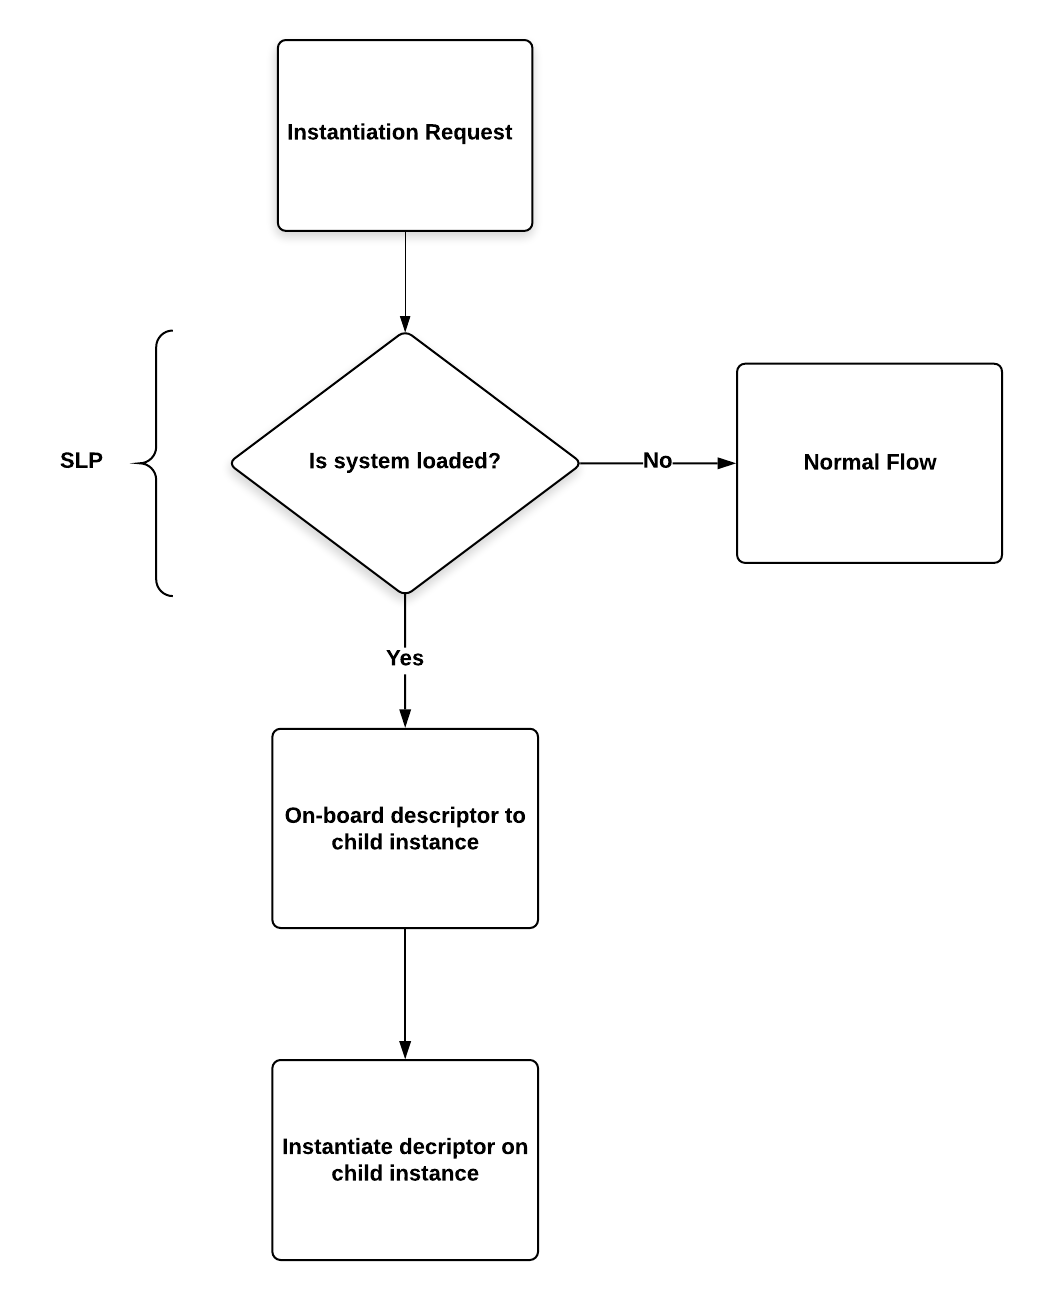
\includegraphics[width=0.8\linewidth]{figures/SLPSLMWorkflow}
	\caption{Service Lifecycle Manager with Scaling Plugin Workflow}
	\label{fig:slpslmworkflow}
\end{figure}

\subsubsection{Scaling Plugin Workflow}

In the figure \ref{fig:splworkflow}, we visualize the rules set of SLP from the List \ref{list:splrules}. SLP is always in the monitoring loop and takes actions according to the system load and the rules set. 

\begin{figure}[h]
	\centering
	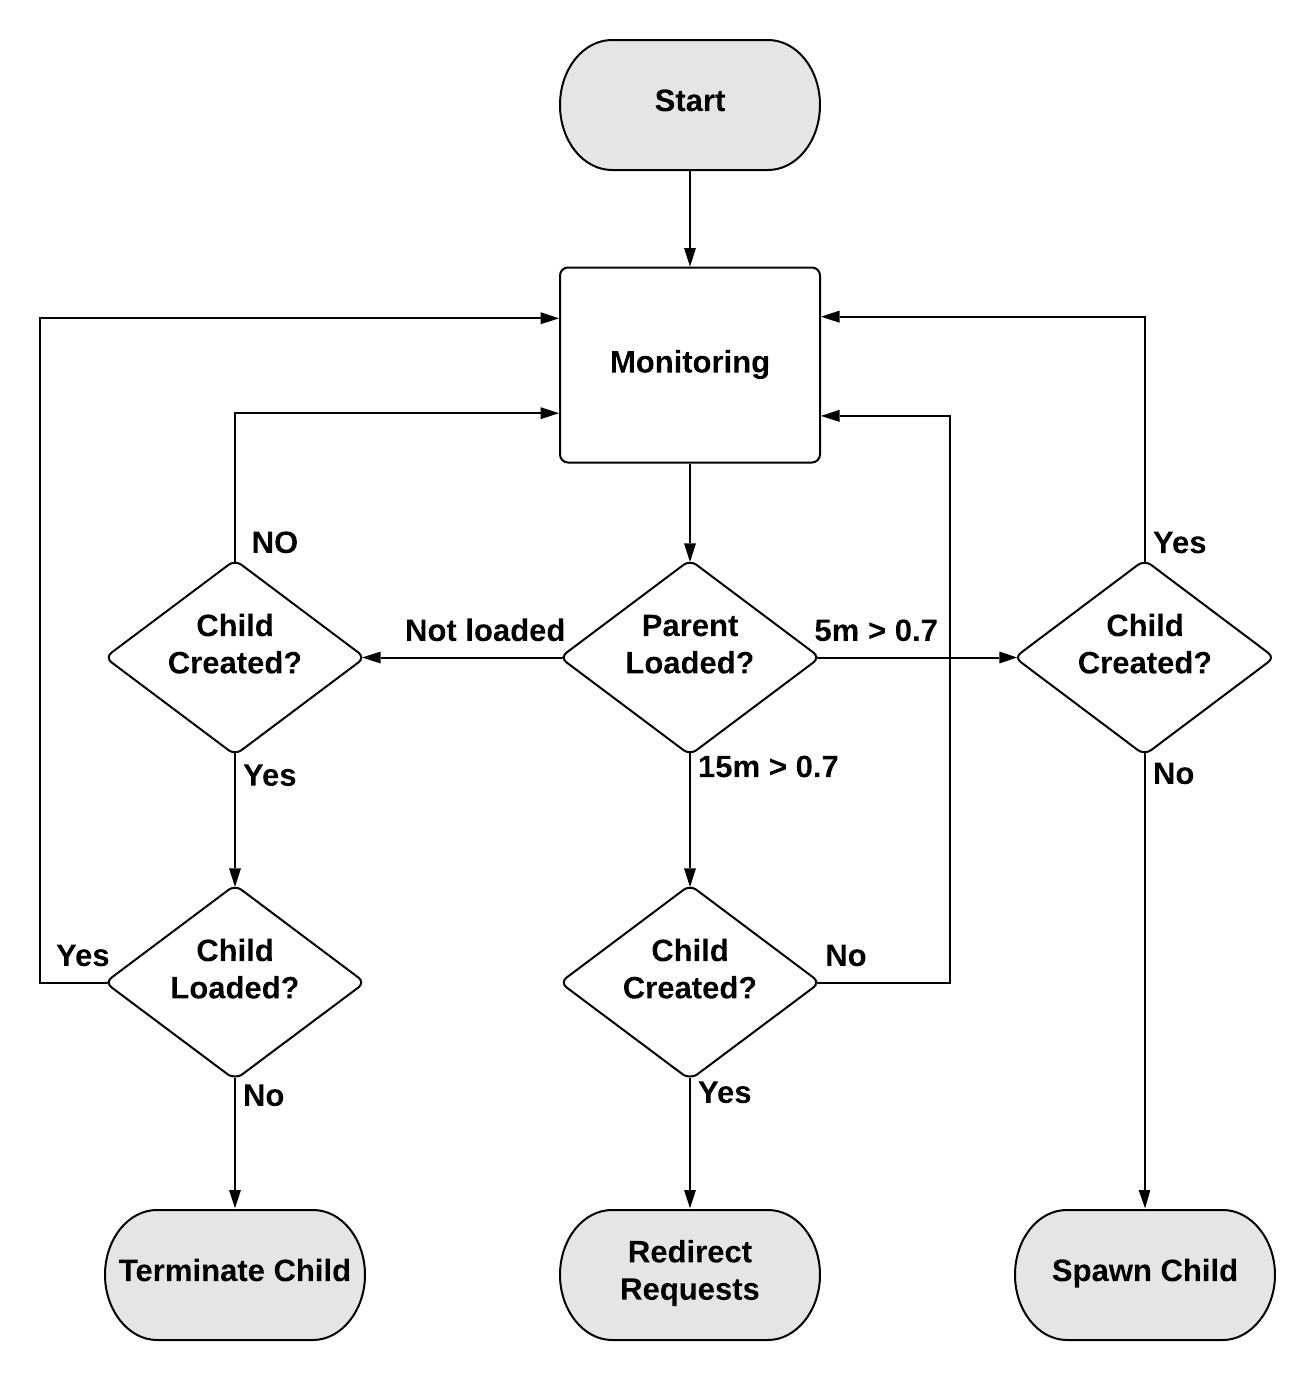
\includegraphics[width=1\linewidth]{figures/SPLWorkflow}
	\caption{Scaling Plugin Workflow}
	\label{fig:splworkflow}
\end{figure}





\section{Experiments}
\todo[inline]{In this section, only talk about the 180 experiment that gave te horizontal graphs}

\subsection{Idea}
\todo[inline]{Here, talk about the idea behind running the experiment and getting to know the docker containers that took the most resources}

\subsection{Testbed}
\todo[inline]{Explain about the machine configuration used to run the experiments, what OS, how many servers and what VIMs where installed, what is the configuration and how python-mano-wrappers were used to send the requests. }

\todo[inline]{Basically explain the whole experiment setup that was used to conduct the experiment.}


\subsection{OSM Results}
The \ref{fig:cirroscase1180-cpu}, \ref{fig:cirroscase1180-mem} and \ref{fig:osm-top-3-lifecycle} shows the CPU utilization, memory utilization and CPU utilization throught the life cycle of the experiment respectively. Let us consider the important dockers in each case and list their functionalities to realize why they have consumed maximum CPU.

\subsubsection{CPU utilization}

The \ref{fig:cirroscase1180-cpu} shows CPU utilization. The first 5 OSM dockers are:

\begin{itemize}
	\item \textbf{osm\_ro:} This is the Resource Orchestrator for OSM. 
	The resource orchestrator is responsible for co-ordinating resource allocation across multiple geo-distributed VIM types.
	It is responsible in processing the resource-allocation requirements of the VNF as per parts of the VNFD and driving the VIM to allocate appropriate compute, network, and storage resources for the deployment of VNFs with their interconnection. 
	
	\item \textbf{osm\_lcm:} This is the Life Cycle Management module for OSM. 
	This docker is responsible for set of operations related to the life cycle of a VNF and NS
	
	\begin{itemize}
		\item \textit{NS LCM operations:} 
		1) On-board Network Service
		2) Instantiate Network Service
		3) Scale Network Service
		4) Update Network Service by supporting Network Service configuration changes
		Create, delete, query, and update of VNFFGs associated to a Network Service.
		5) Terminate Network Services
		
		\item \textit{VNF LCM operations:} 1) Instantiate VNF (create a VNF using the VNF on-boarding artefacts)
		2) Scale VNF (increase or reduce the capacity of the VNF).
		3) Update and/or Upgrade VNF (support VNF software and/or configuration changes of various complexity).
		4) Terminate VNF (release VNF-associated NFVI resources and return it to NFVI resource pool)
	\end{itemize}
	
	
	
	\item \textbf{osm\_mon:} This is the monitoring module for OSM. 
	The main task of this docker is to retreive metrics from VIM. 
	It keeps polling VIM every 30 seconds. 
	
	\item \textbf{osm\_ro\_db:} This is called RO database module.
	RO module in OSM maintains its own database called ro-db. (RO module is usually edited to enable or disable this particular module)
	This module takes care of database related operations. According to the osm/ro.git, ro-db stores different IDs like vnfd id ,osm id, tenant id, vim id etc. There is something called scenario. ro db stores these scenarios and scenario ID and then a scenario gets executed when the scenario id matches with the right tenant id, osm id and vnfd id. 
	It stores vim actions, wim actions and they are processed sequentially. 
	
	\item \textbf{osm\_nbi:} North Bound Interface of OSM. Restful server that follows ETSI SOL005 interface.
	It is the unique entry point for all the interactions with the OSS/UI system.
	This serves as the interface for MANO operations.
	(OSM's NBI offers all the necessary abstractions to allow clients for the complete control, operation and supervision od the NS.)
\end{itemize}

\begin{figure}[h]
	\centering
	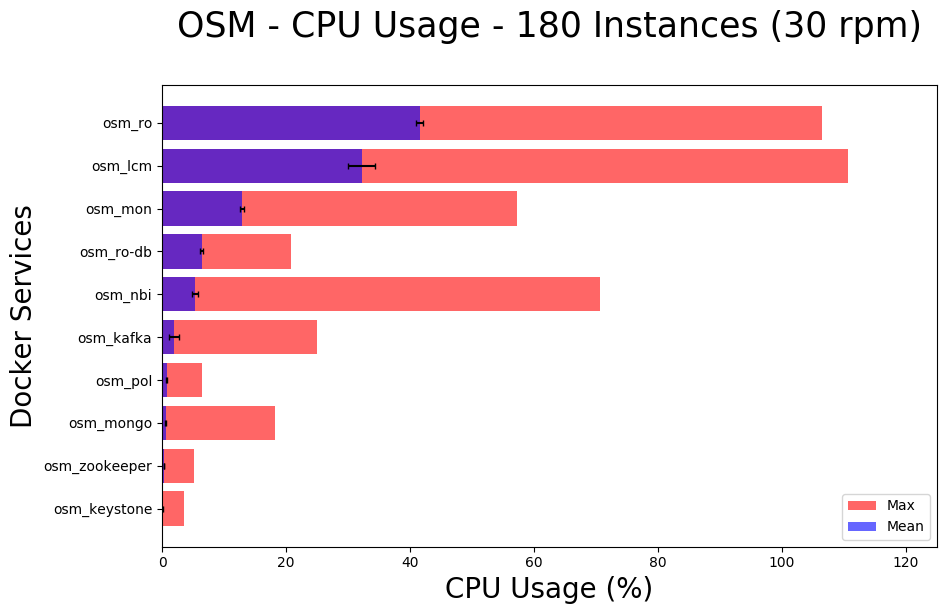
\includegraphics[width=0.7\linewidth]{../figures/scalability_graphs/Horizontal-Docker-Graphs/osm/cirros_case1_180-CPU}
	\caption{OSM CPU}
	\label{fig:cirroscase1180-cpu}
\end{figure}

\pagebreak



\subsubsection{Memory Utilization}

The first 5 OSM dockers in memory utilization graph are:

\begin{itemize}
	\item \textbf{osm\_mongo:} This is a common non relational database for OSM modules.
	\item \textbf{osm\_kafka:} This module provides a Kafka bus used for OSM communication.
	\item \textbf{osm\_nbi:} This is the north bound interface for OSM module. The functionalities of this module remains the same(as explained in the previous subsection)
	
	\item \textbf{osm\_light-ui:} This docker is an implementation of a web GUI to interact with the Northbound API. (The framework allows editing, validating, visualizing the descriptors of services and components both textually and graphically)
	\item \textbf{osm\_ro\_db:} This is the RO database. The functionalities of this module remains the same (as explained in the previous subsection)
	
\end{itemize}



\begin{figure}[h]
	\centering
	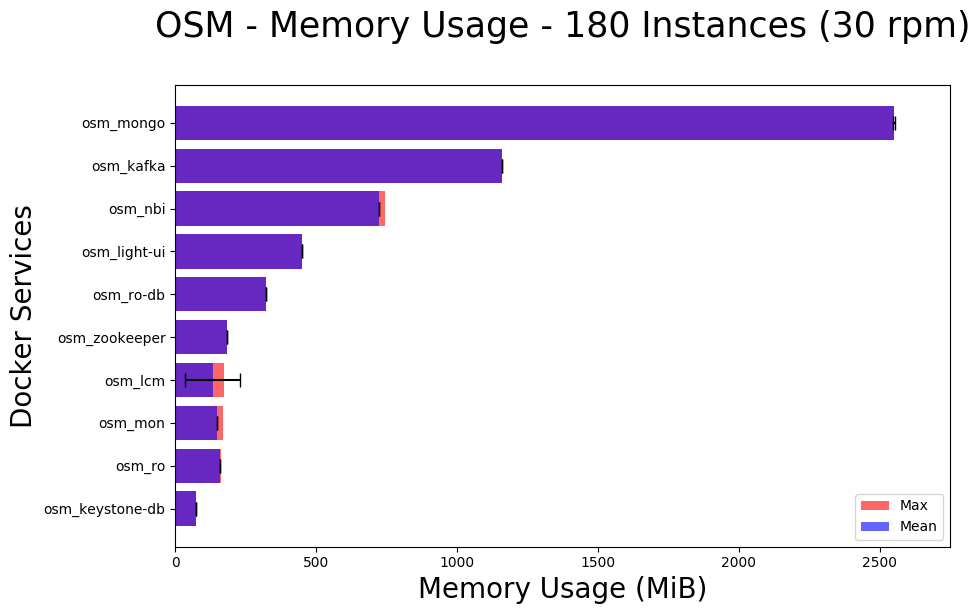
\includegraphics[width=0.7\linewidth]{../figures/scalability_graphs/Horizontal-Docker-Graphs/osm/cirros_case1_180-MEM}
	\caption{OSM MEM}
	\label{fig:cirroscase1180-mem}
\end{figure}


\subsubsection{Lifecycle}

We now have the life cycle graphs of the entire experiment. This shows the distribution of the CPU usage among the top 3 dockers throughout the experiment. The experiment lasted for about 10 minutes.

We can observe that the ro module of OSM got continuous requests over the time and at the end all the termination requests came at once. Also LCM , mon modules continously processed the requests. mon module retrieved metric information continuously and the same trend
remains throughout the experiment.

\begin{figure}[h]
	\centering
	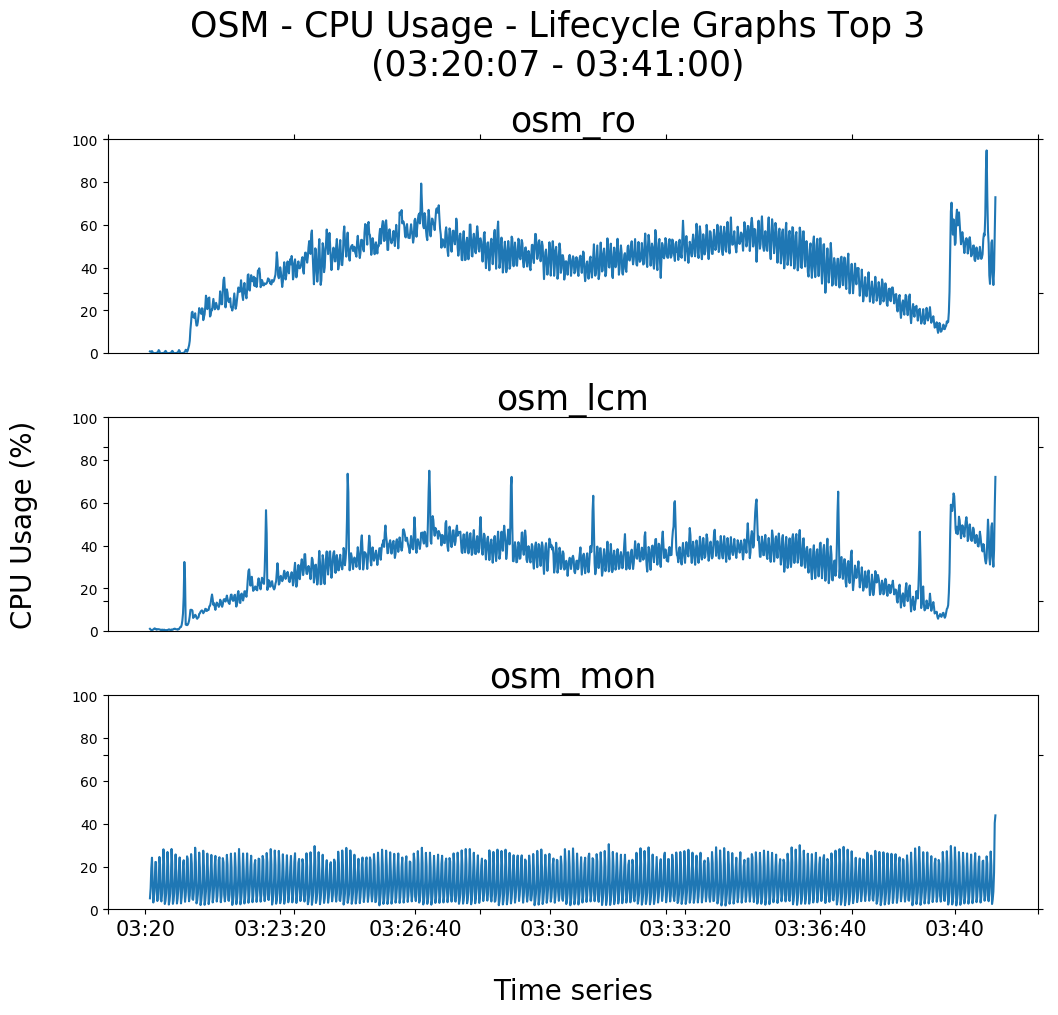
\includegraphics[width=0.7\linewidth]{figures/scalability_graphs/Lifecycle-Graphs-Top-3/OSM-TOP-3-Lifecycle}
	\caption{OSM LS}
	\label{fig:osm-top-3-lifecycle}
\end{figure}


\subsection{Pishahang Results}
\todo[inline]{Pishahang Just like you did in the presentation, explain the functionalities of the top 5 dockers and why they are taking}

\subsubsection{CPU}

\begin{figure}[h]
	\centering
	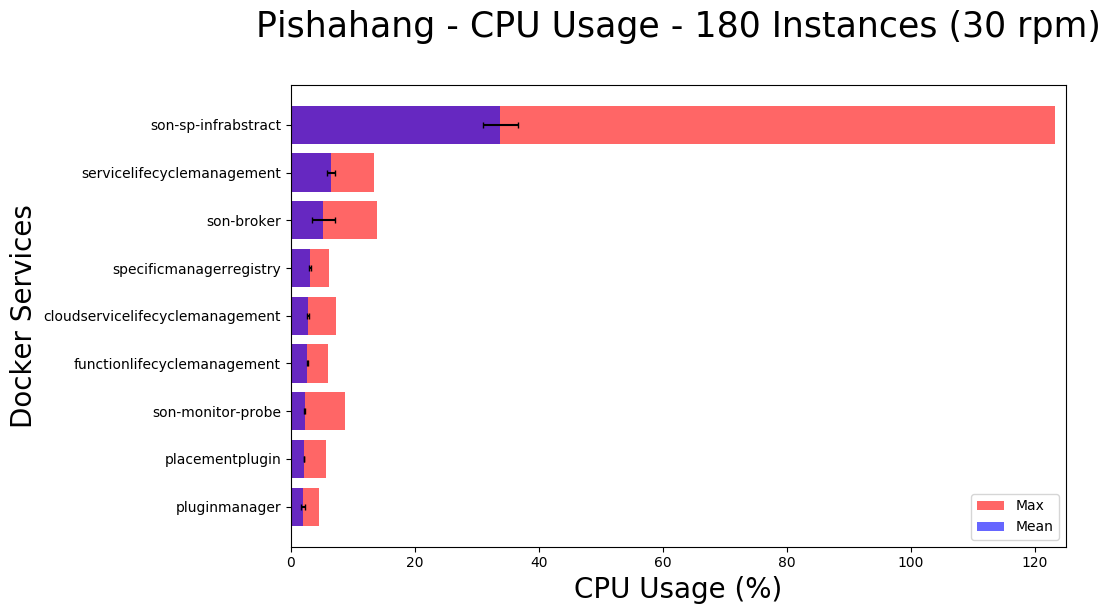
\includegraphics[width=0.7\linewidth]{../figures/scalability_graphs/Horizontal-Docker-Graphs/pishahang/cirros_case1_180-CPU}
	\caption{Pishahang CPU}
	\label{fig:pishcirroscase1180-cpu}
\end{figure}

\subsubsection{Memory}

\begin{figure}[h]
	\centering
	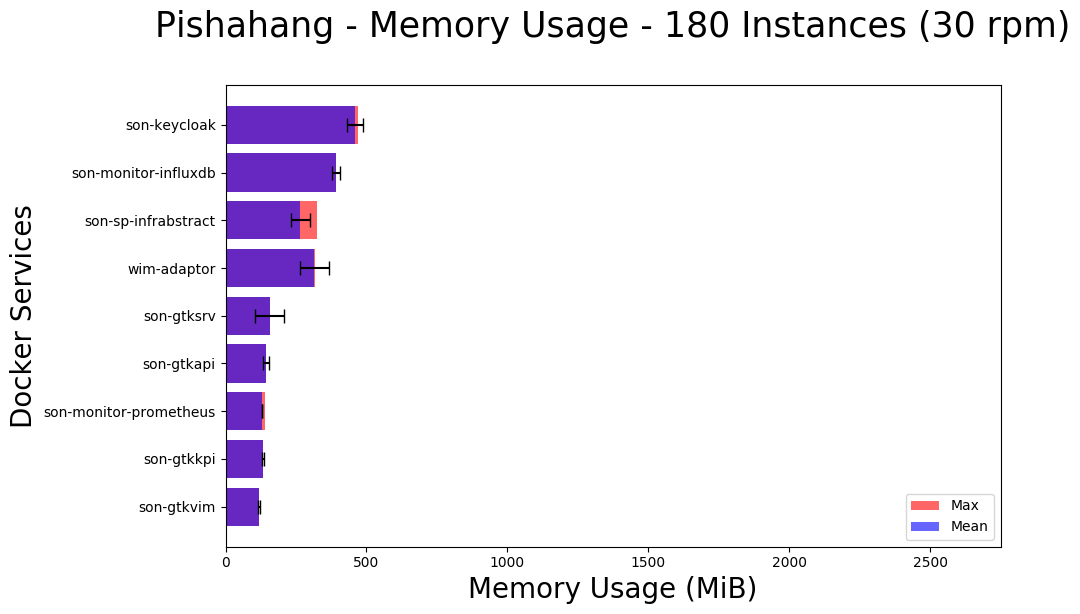
\includegraphics[width=0.7\linewidth]{../figures/scalability_graphs/Horizontal-Docker-Graphs/pishahang/cirros_case1_180-MEM}
	\caption{Pishahang MEM}
	\label{fig:pishcirroscase1180-mem}
\end{figure}


\subsubsection{Lifecycle}

\begin{figure}[h]
	\centering
	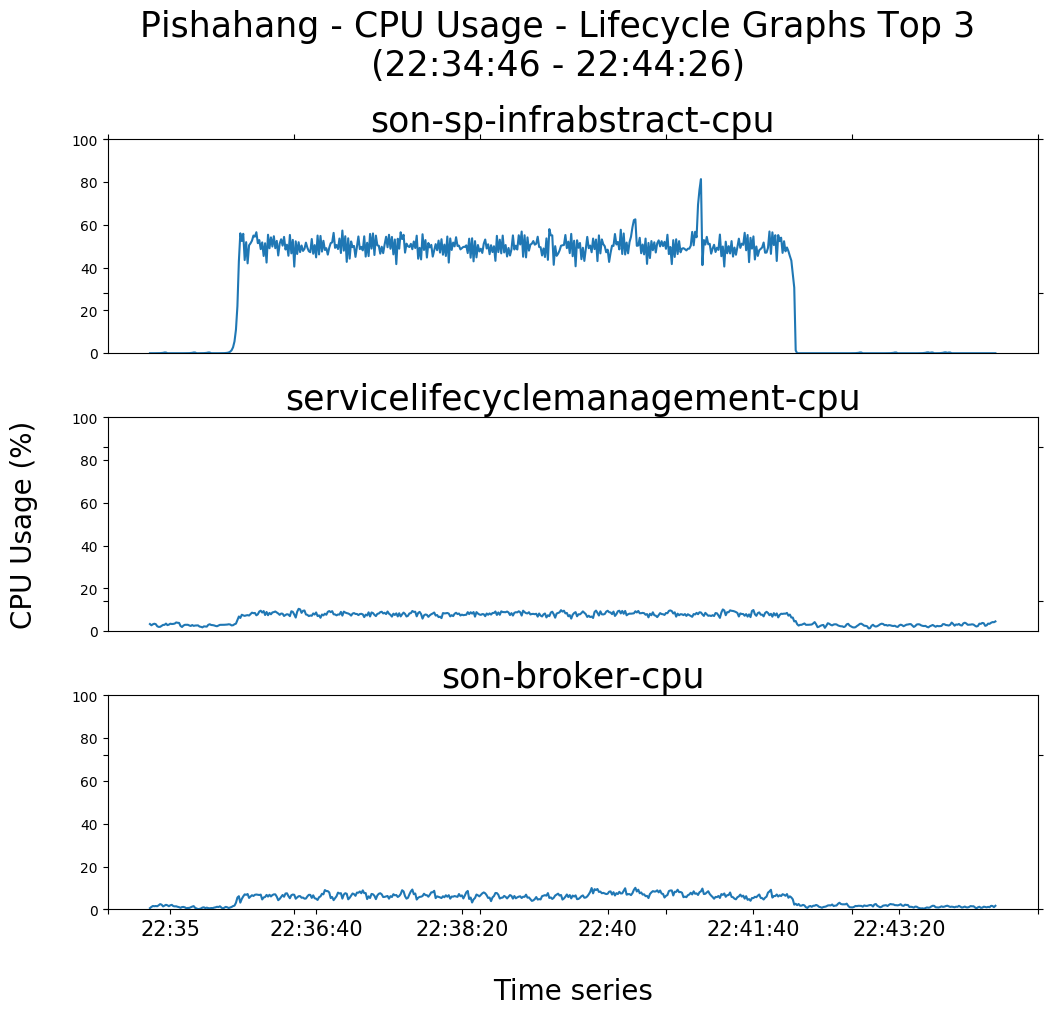
\includegraphics[width=0.7\linewidth]{figures/scalability_graphs/Lifecycle-Graphs-Top-3/Pishahang-TOP-3-Lifecycle}
	\caption{Pish LS}
	\label{fig:pishahang-top-3-lifecycle}
\end{figure}



\subsection{Summary of issues of the experiment}
\todo[inline]{Blockers: VIM support issues, openstack not stable, k8 not supported in OSM. Why 180. RPM issues}
	
\subsection{Inference from the experiment} 
\todo[inline]{about identifying the top dockers, some more info about the lifecycle graphs}

\section{MANO Benchmarking Framework} 

\subsection{Introduction}

MANO Benchmarking Framework (MBF) is a result of a small script that was used to run the experiments discussed in the previous sections. 
The idea of MBF is to provide MANO developers with a generic framework for running experiments on MANO. 
MBF mainly provides the following 1) Easy interfacing with MANO instances by using python-mano-wrappers, 2) Ability to run experiments with different service descriptors, 3) Collection of performance metrics in convenient data format and 4) Flexible graphing mechanism of the collected data. 


\subsection{Design}

MBF is designed for ease of use and low barrier to entry for developers. 
We explain the choice of tools that are used in MBF in the following list.

\begin{itemize}
	\item{\textbf{Netdata\footnote{https://github.com/netdata/netdata}}} is the metrics monitoring system for MBF. 
	Netdata captures relevant system metrics and provide powerful APIs to query the recorded data in a suitable format.
	\item{\textbf{Python}} as the choice of scripting language was obvious as the MANOs itself are implemented in python.
	\item{\textbf{python-mano-wrappers}} is used to provide access to REST APIs of MANOs from python.
	\item{\textbf{Docker}} is used to containerize MBF, thus making it easy to distribute and portable.
	\item{\textbf{Matplotlib}} is the graphing library for MBF due to its flexibility and ease of use.
	\item{\textbf{Flask}} as a python server that can be used to provide additional interactions with the experiment runner.

\end{itemize}


\subsection{Parameters and KPIs} 

\subsubsection{Parameters}

MBF has experiment parameters that can be altered. 
The following paramenters are supported

\begin{itemize}
	\item{\textbf{Descriptors}} NSDs and VNFDs can be changed. 
	a list of NSDs/VNFDs is also supported. 
	When a list of descriptors are provided, the experiment will be run for each of the descriptors.
	\item{\textbf{Number of instances}} Total number of instantiation requests to be sent to the MANO.
	\item{\textbf{Number of runs}} number of re-runs of the same experiment to be run. 
	This is performed to measure the variance in results.
	\item{\textbf{Requests per minute (RPM)}} The rate at which the instantiation requests are sent to the MANO
	\item{\textbf{Observation Time}} The observation time after the instantiation requests are sent. 
	This can be used to collect metrics post instantiation to observe how MANO behaves in the monitoring phase.
	\item{\textbf{Inter-experiment Delay}} is the time between experiment runs. 
	This is altered to give enough time for the VIM to terminate and cleanup instances from the previous experiment runs if any.
	\item{\textbf{Skip experiment on error}} if set to true, the current run is skipped due to a failed instance on the VIM.

\end{itemize}

\subsection{Key Performance Indicators}

MBF stores resource utilization metrics during the experiment and generates graphs to visualize the results. 
However, these are only examples and the further possibilities are supported by the framework. 
The metrics are stored as CSV files.

\begin{itemize}
	\item{\textbf{CPU}} Overall system CPU usage is recorded as well as the individual docker micro service CPU usage metrics are stored.
	\item{\textbf{Memory}} Overall system memory usage along with the individual docker micro service memory usage is stored.
	\item{\textbf{System Load}} The 1m, 5m and 15m moving averages of system load values provided by the linux kernel is stored.
	\item{\textbf{Status Tracking}} The status of all instances are stored by polling the VIM every 5 seconds over the experiment lifetime. 
	This enables to track the status change over time.
	\item{\textbf{End-to-end Deployment Time}} is the time elapsed to deploy all the instances on the VIM.
	\item{\textbf{Individual Deployment Time}} is the time taken by each instance for deployment. 
	This is also split into time taken by MANO and VIM.
\end{itemize}

\subsection{Steps for experiment run} 

The steps to run a basic experiment is detailed in this section. 
The following instruction is to run an experiment with 90 instances on OSM using an network service with 1 VNF. 

\begin{enumerate}
	\item Git clone the experiments-branch\footnote{https://github.com/CN-UPB/MANO-Benchmarking-Framework}
	\item Build and start the docker container
	\item Change experiment variables in the relevant scripts for respective MANOs
	\begin{itemize}
		\item \textbf{OSM} -- \textit{run-experiment-osm.py}
		\item \textbf{Sonata (Pishahang)}  -- \textit{run-experiment-sonata.py}
		\item \textbf{Sonata Container Orchestration (Pishahang)} -- \textit{run-experiment-sonata-k8}
	\end{itemize}
	
	\item Run the relevant script from inside the container. 
	The experiment will now run and stores result files in the same directory
	\item Use the result parser from the \texttt{experiments/results/csv-result-parser.py} to parse the results and store it in a format suitable for graphing
	\item Use the graph plotter on the parsed files to generate the graphs\\ \texttt{experiments/results/plot-graphs.py}
	
	\end{enumerate}

The commands required to run these are listed in the readme file here, \\ \url{https://github.com/CN-UPB/MANO-Benchmarking-Framework/blob/master/README.md}

\textit{\\\textbf{Note:} This process is being streamlined to reduce some redundant steps and will be released in the next version of MBF.} 

\subsection{Example Use Cases}

In this section we demonstrate a few use cases of MBF. 
The framework facilitated easy experimentation, collection and analysis of metrics in the following cases. 
However, in-depth analysis of what the metrics and graphs mean are out of scope of this document. 



\subsubsection{Comparison of different network services} 

We compared the performance metrics of different NSDs/VNFDs and visualized it. 
For this, we provided 6 different network service descriptors to the experiment runner. 
First 3 NS consisted of a cirros image as a VNF with 1, 3 and 5 VNFs per NSD and the other 3 NS consisted of an ubuntu image as a VNF with 1, 3 and 5 VNFs per NSD.\\

The experiment stores the KPIs listed in the previous section, along with the graphs visualizing the differences. 
This graph is produced for each micro-service showing the resource utilization of each NS under different number of instantiations. 
As an example, the figures \ref{fig:osmlcm-mean-cpu-cases} and \ref{fig:osmro-mean-cpu-cases} show the CPU utilization of the OSM microservice LCM and RO respectively.

\begin{figure}[h]
	\centering
	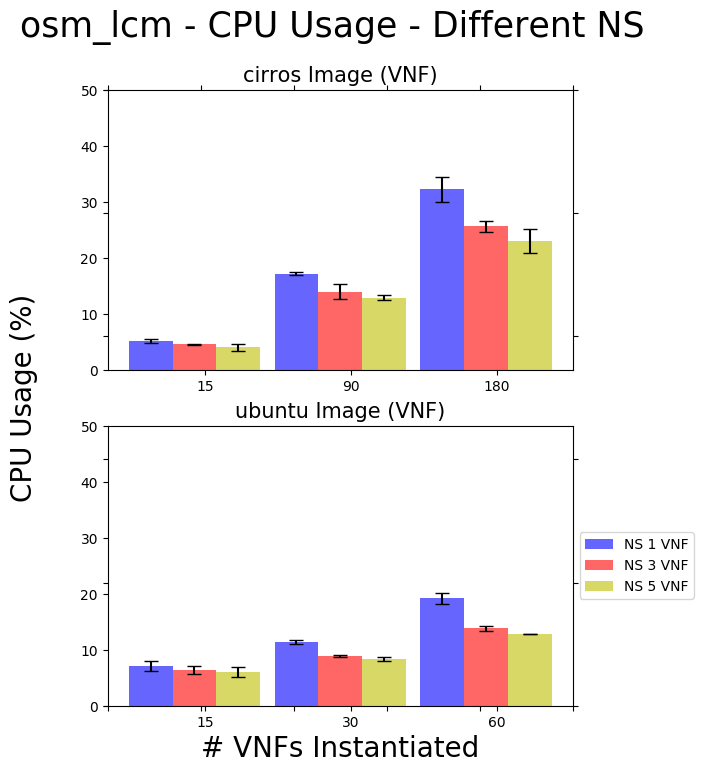
\includegraphics[width=0.6\linewidth]{figures/scalability_graphs/Docker-Grouped-Cases/osm/osm_lcm-Mean-CPU-Cases}
	\caption{CPU usage of OSM microservice LCM}
	\label{fig:osmlcm-mean-cpu-cases}
\end{figure}

\begin{figure}
	\centering
	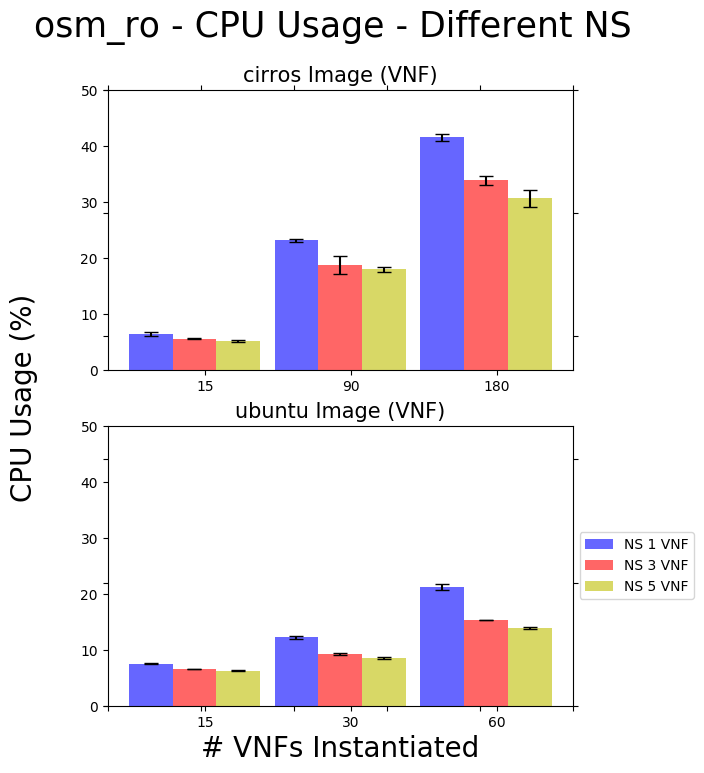
\includegraphics[width=0.6\linewidth]{figures/scalability_graphs/Docker-Grouped-Cases/osm/osm_ro-Mean-CPU-Cases}
	\caption{CPU usage of OSM microservice RO}
	\label{fig:osmro-mean-cpu-cases}
\end{figure}

\pagebreak

\subsubsection{Container vs VM Orchestration} 

Pishahang supports container orchestration on kubernetes and OSM supports VM orchestration on OpenStack. 
We compared the performance of orchestrating similar network services on VM and containers. 
In the figure \ref{fig:timecomparison}, the graph on top shows the average time distribution between MANO and VIM for deploying one network service with one VNF. 
The bottom graph in the figure \ref{fig:timecomparison} shows the total time taken to deploy 90 instances of a network with one VNF. 
The time taken to deploy similar VNFs is significantly less for containers, which is expected as containers are light weight compared to a VMs. \\

\textit{Note:} Pishahang support for VM orchestration is not stable, hence, we could not perform similar VM experiments on Pishahang for this comparison.

\begin{figure}[h]
	\centering
	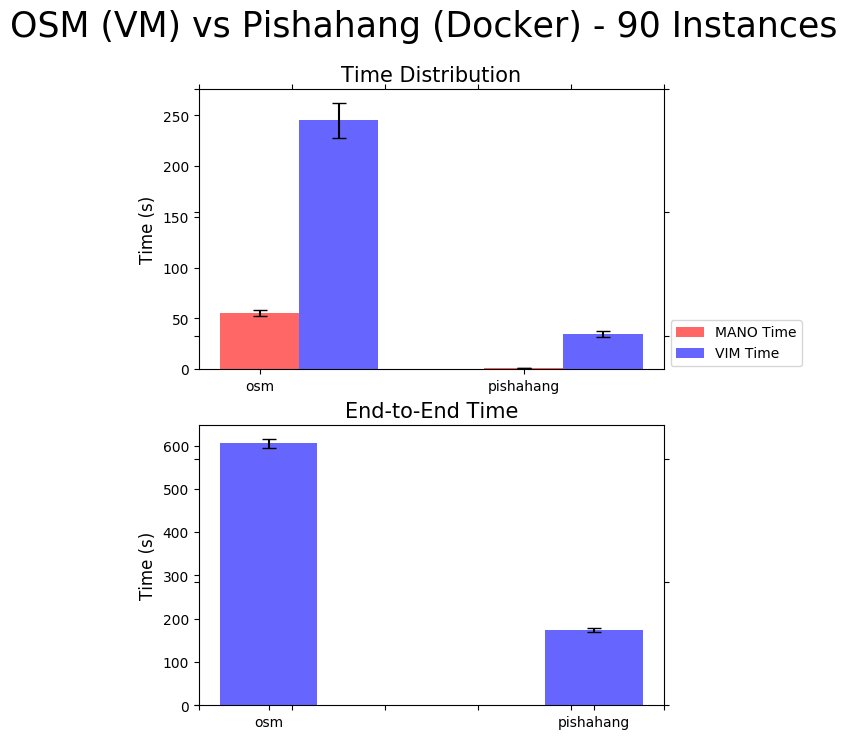
\includegraphics[width=0.7\linewidth]{figures/scalability_graphs/Comparison-VM-Docker/Time_comparison}
	\caption{Time distribution in MANO and VIM}
	\label{fig:timecomparison}
\end{figure}


\begin{figure}[h]
	\centering
	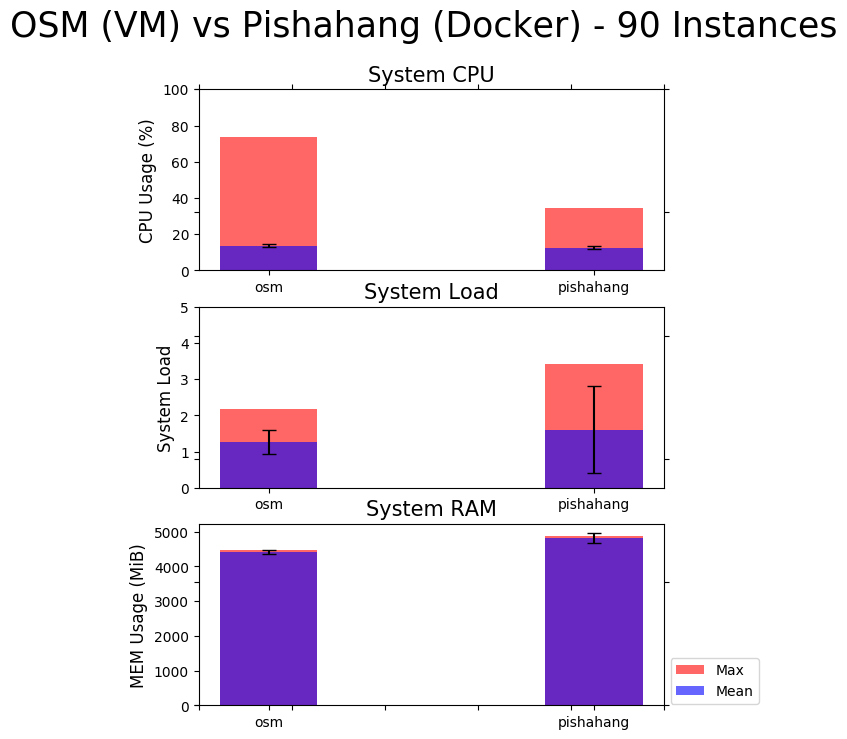
\includegraphics[width=0.7\linewidth]{figures/scalability_graphs/Comparison-VM-Docker/System_metrics_comparison}
	\caption{System resource utilization}
	\label{fig:systemmetricscomparison}
\end{figure}




\subsubsection{Scaling Plugin Evaluation}

We utilized MBF to evaluate our Scaling Plugin discussed in the section \ref{scalingplugin}. 
The Parent Pishahang instance is running the scaling plugin in debug mode, which can be used to mock system load values. 
We added a REST call to the MBF flask server to mock the system load values in the scaling plugin.\\

The experiment was designed to instantiate 90 instances of  cirros docker containers on Pishahang. 
After sending 30 instantiation requests, the experiment script alters the \textit{5m} system load to greater than 0.7, which triggers Rule 1 from the SLP rule set \ref{list:splrules}. 
Thus, creating a new child Pishahang instance. 
However, in the debug mode, for the scope of this experiment, we had a child instance already instantiated from start.\\

After instantiating 45 instances, the script mocks the \textit{15m} system load value to greater than 0.7, which triggers Rule 2 from the SLP rule set \ref{list:splrules}. 
Thus, parent instance will now redirect any further service requests (i.e., 46th instantiation requests on-wards) to the child Pishahang instance.

We use the overall lifecycle data collected by MBF to visualize the CPU usage over time of the top 3 microservices (based on CPU usage).\\

The experiments ran from 11:17:02 to 11:28:23. 
Initially the microservices on the parent instance took all the load, as it can be seen from the figure \ref{fig:parent-top-3-lifecycle}. 
At about the half way mark, the requests are redirected to the child instance. 
The load distributed to the child instance can be seen in the figure \ref{fig:child-top-3-lifecycle}. 


\begin{figure}
	\centering
	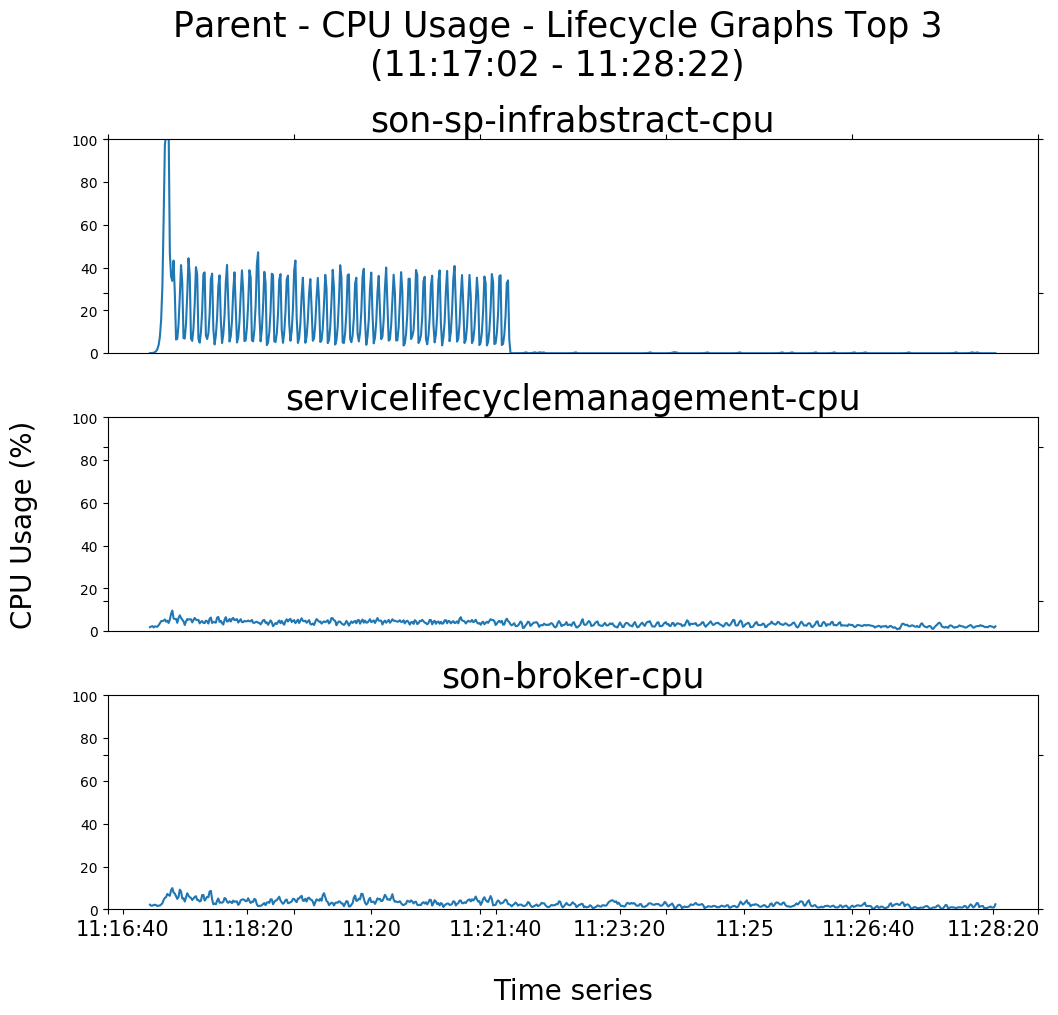
\includegraphics[width=0.65\linewidth]{figures/scalability_graphs/Scalability-Evaluation/Parent-TOP-3-Lifecycle}
	\caption{Parent MANO instance lifecycle graph}
	\label{fig:parent-top-3-lifecycle}
\end{figure}

\begin{figure}
	\centering
	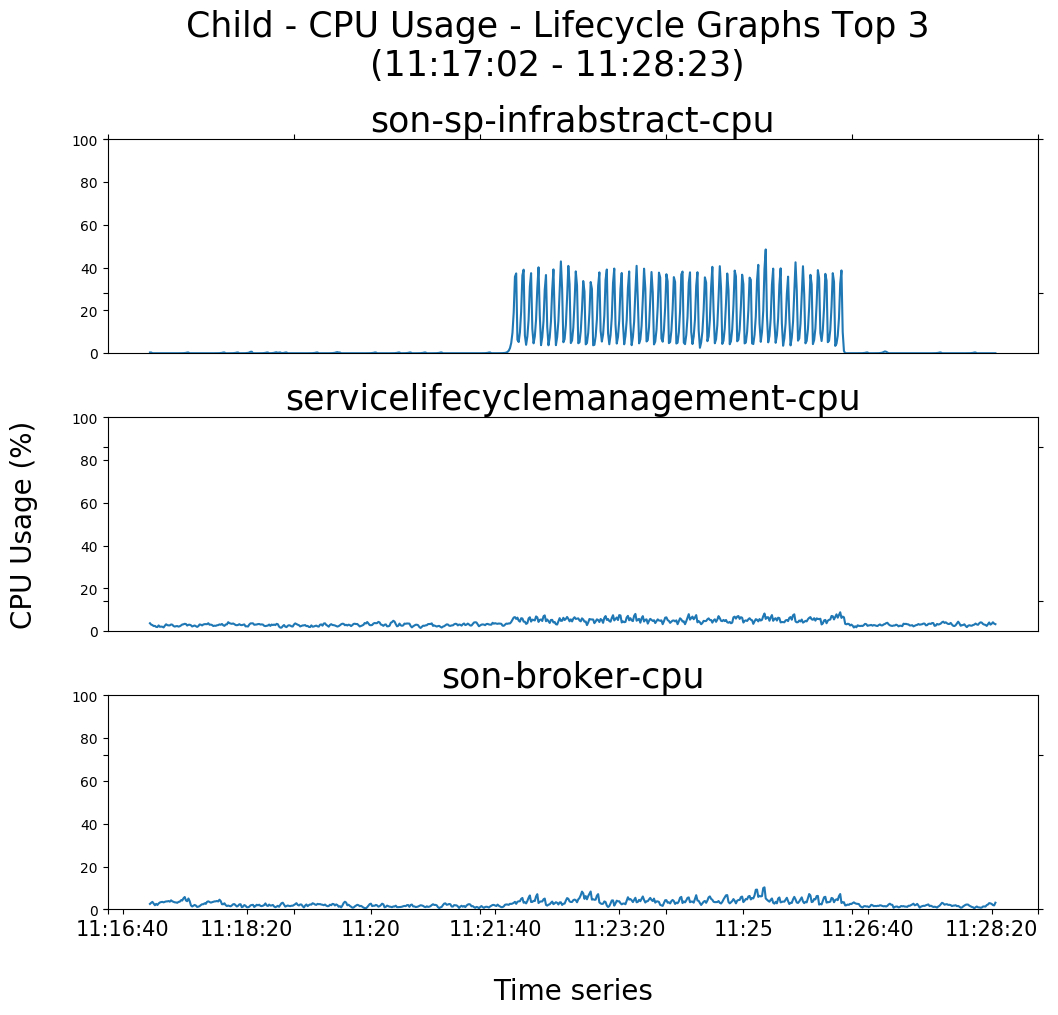
\includegraphics[width=0.65\linewidth]{figures/scalability_graphs/Scalability-Evaluation/Child-TOP-3-Lifecycle}
	\caption{Child MANO instance lifecycle graph}
	\label{fig:child-top-3-lifecycle}
\end{figure}



\subsection{Future scope}
\todo[inline]{TODO: scope of MBF}

\pagebreak

\section{Discussions}

In this section, we discuss the 

\subsubsection{RPM and success ratio}
\subsubsection{NSDs with different number of VNFDs}
\subsubsection{Different VNFs}
\subsubsection{Container v/s VM}
\begin{itemize}
	\item Time distribution
	\item System metrics
\end{itemize}

